\section{Deniable Signature Key Exchange}

\begin{frame}
  \frametitle{DSKE}
  This subprotocol constructs an association table between participants and the keys they will use for message signing.\\[0.3cm]

  Any information transmitted during this protocol is:

  \begin{itemize}
    \item Authenticated
    \item Deniable
  \end{itemize}

  This would be the image of the chat room just after the DSKE is finished:
  \begin{figure}
    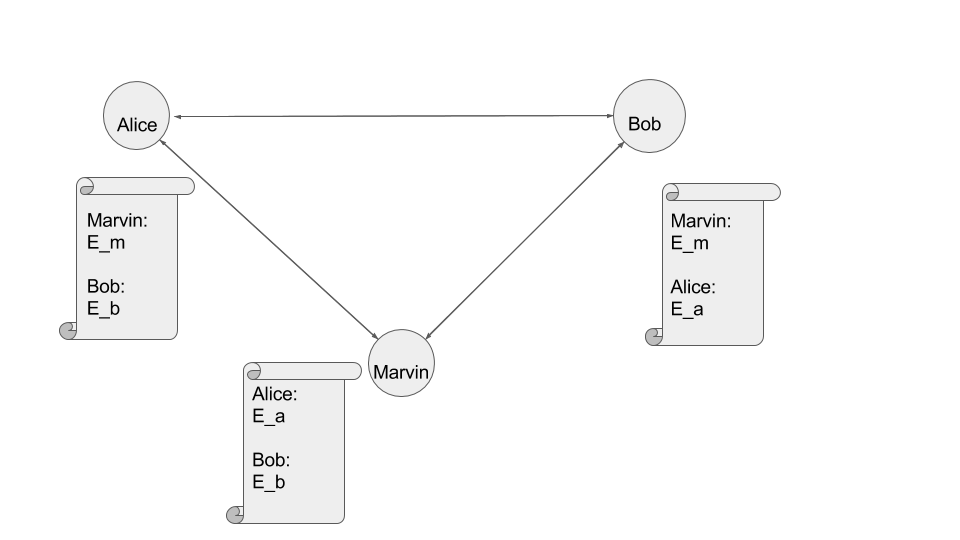
\includegraphics[scale=0.2]{Figures/denAKE.png}
  \end{figure}
\end{frame}

\begin{frame}
  To achieve that, DSKE assumes the existance of a subprotocol called \emph{Deniable Authenticated Key Exchange} (denAKE).\\[0.3cm]

  The denAKE protocol creates an {\bf authenticated} and {\bf deniable} shared secret between two participants. Using that shared secret the two participants send each other the public key they will be using. This is done for every pair of participants.\\[0.3cm]

  \begin{minipage}{.47\textwidth}
    In our implementation denAKE is implemented using the triple diffie hellman where the shared secret is:

    \[
      s = g^{Xy} || g^{xY} || g^{xy}
    \]

  \end{minipage}
  \begin{minipage}{.47\textwidth}
     \begin{figure}
      \scalebox{0.5}{ \begin{tikzpicture}

  \def \dist {5cm}
  \def \longrad {1cm}
  \def \ephemrad {0.8cm}
  \def \sqrttwo {1.4142}

  \node[draw, circle, minimum size=\longrad] at (0,\dist) {$X$};
  \node[draw, circle, minimum size=\ephemrad] at (0,0) {$x$};
  \node[draw, circle, minimum size=\longrad] at (\dist,\dist) {$Y$};
  \node[draw, circle, minimum size=\ephemrad] at (\dist,0) {$y$};

  \draw[<->, >=latex] ({0 + (\sqrttwo * \longrad / 4)} ,{\dist  - (\sqrttwo * \longrad / 4)})
  -- ({\dist - (\sqrttwo * \ephemrad /4)},{0 + (\sqrttwo * \ephemrad / 4)});

  \draw[<->, >=latex] ({\dist - (\sqrttwo * \longrad / 4)} ,{\dist  - (\sqrttwo * \longrad / 4)})
  -- ({0 + (\sqrttwo * \ephemrad /4)},{0 + (\sqrttwo * \ephemrad / 4)});

  \draw[<->, >=latex] ({0 + \ephemrad/2}, 0) -- ({\dist - \ephemrad/2}, 0);

\end{tikzpicture}
}
    \end{figure}
  \end{minipage}
\end{frame}
